%!TEX root = ../projecto.tex

\section{Architecture} % (fold)
\label{sec:architecture}
This section is comprised of the multiple layers needed in order to successfully be able to implement the proposed project objectives. We will discuss the data gathering process, and detail the SOM algorithms that will be tried in order to achieve the best results on Topic Detection in Twitter. The description of the evaluation method will be described and finally the prototype architecture will be described.

\subsection{Collecting Data} % (fold)
\label{sub:data_gathering}
For this project we will focus on building our own  dataset for SOM training, but existing datasets might be used in order to rate results. The description of existing datasets will be presented in Subsection~\ref{sub:testing_for_precision_and_recall}. 

\subsubsection{Twitter API} % (fold)
 \label{ssub:building_a_data_set}
 Building your own Data Set through the Twitter API has become harder with passing years with the introduction of API limits and mandatory authentication. With these new limitations, companies like \emph{Gnip} \footnote{http://gnip.com/topsy/} or \emph{Tweet Archivist} \footnote{http://www.tweetarchivist.com/about/subscriptions} with licenses from Twitter are selling access to their archives of tweets.

 In order to retrieve data from Twitter is crucial to understand how their API functions. The Twitter API right now is divided into two types, the REST API and the Streaming API. Both can be used at the same time, and have different types of limits. In a general way, the streaming API is used for subscriptions, where a an application can subscribe a given hashtag or user activity on the social network, and they are automatically pulled to the subscriber app. The Streaming API has no specific limit being described in the docs as ``The public streaming APIs cap the number of messages sent to your client to a small fraction of the total volume of Tweets at any given moment" \footnote{https://dev.twitter.com/docs/faq\#6861}.

 The REST API works by requesting resources and getting the results in a RESTful way. Here the limits are strict, an application cat only get a maximum number of 3200 Tweets per user and 180 calls to the API per 15 minutes, more API limits can be found on the Twitter API Documentation \footnote{https://dev.twitter.com/docs/rate-limiting/1.1/limits}.
 % subsubsection building_a_data_set (end) 

\subsubsection{Crawling Twitter} % (fold)
\label{sub:crawling_twitter}
In order to get tweets from the Twitter API, the data will be crawled in a breath-first fashion where after selecting a first user:

\begin{itemize}
  \item Get all Tweets from the user.
  \item Get user profile info.
  \item Get list of followers/followees.
  \item Select a follower/followee and repeat step one.
\end{itemize}

The algorithm will stop at a given depth level, also if API limits are exceeded the algorithm will have to stop for 15 minutes and afterwards resume. Given the API access limits, there will be no need to run the crawler asynchronously since achieving a greater level of performance will only make the algorithm achieve API limits sooner.
% subsubsection crawling_twitter (end)

\subsubsection{Storing Crawled Data} % (fold)
\label{sub:storing_crawled_data}
While the crawler is getting data from Twitter, it will be storing it in a Redis database \footnote{http://redis.io/}. Given the amount of databases available in last few years, Redis was chosen for this project because it met the following criteria:
\begin{itemize}
  \item Free.
  \item Simple to install and run. 
  \item Can persist data to disk.
  \item Its really fast to write, by not granting data integrity (which is not a problem since this project is not dealing with sensitive information)
  \item Good documentation.
  \item Non relational, Key/Value store.
  \item Stores json.
  \item Client libraries for almost every programing language.
  \item Integrated publish/subscriber.
\end{itemize}

Given the characteristics of the Redis database, there will be no need to write a schema beforehand. With this in mind, user information and Tweets will be stored directly in json into the Database.
% subsubsection storing_crawled_data (end)
% subsubsection data_gathering (end)

\subsection{The SOM Algorithm} % (fold)
\label{sub:implementing_the_som}
The SOM algorithm in this report will have a twofold approach. Primarily we will try to transform the tweet social characteristics and words into a vector using the vector space model, this approach will use the default SOM implementation and will be described in detail in Subsection~\ref{ssub:default_som_approach_}. The second approach is inspired by~\citet{Bacao2005} where the SOM algorithm will be altered in order to take in consideration the social network during the its training, this implementation will be described in Subsection~\ref{ssub:social_som}.
% subsection implementing_the_som (end)

\subsubsection{Default SOM Approach } % (fold)
\label{ssub:default_som_approach_} In order to train the SOM first we will need to convert the tweets into the vector space model. There will be two binary vectors, the first one will represent the presence of all the words gathered in all tweets where the value 1 will  represent the presence of a word and the value 0 the absence of a word. The second vector will represent the social connections between the user. On a first approach, in order to  give more relevance to social connections, only followers that are followed back will be represented. This approach will give a stronger representation to the social interaction between the two users, since on the Twitter social network it possible to follow someone without the followed person accepting the request. In the end both vectors, the word representation vector and the social connections representation vector will be concatenated. Figure~\ref{fig:vsm} shows the transformation from the tweet into the vector space model. 

\begin{figure}[tb]
  \begin{center}
    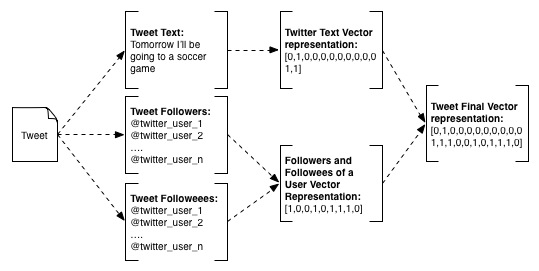
\includegraphics[width=9cm]{images/10_tweet_svm_transform.jpg}
  \end{center}
  \caption{Vector Space transformation of a Tweet}
  \label{fig:vsm}
\end{figure}

The SOM initialization will be tried in different ways and measured to see which gives the best results. The initialization characteristics will be the following:
\begin{itemize}
  \item Random initial number of neurons with random content.
  \item Random initial number of neurons with random content evenly distributed.
  \item Each neuron will be the representation of each user that was crawled.
  \item Each neuron will be comprised of words relevant to a determined topic, and will be responsible to categorize that topic.
  \item Each neuron will be the representation of a user that is relevant to determined topic, for example the user \emph{Optimus Alive} would be responsible for categorizing the topic \textit{"Music Festivals"}  while \emph{Cristiano Ronaldo} neuron representation would be responsible for detecting the topic \emph{Soccer}.
\end{itemize}

In the initializations described above, only the last two will yield a SOM ready to classify tweets into topical categories. The first three options would build uncategorized clusters that would have to be classified \emph{a posteriori}. Nevertheless it will be important to look at the results given by them because they could be more interesting then the results from the last two items.
% subsubsection default_som_approach_ (end)

\subsubsection{Social SOM} % (fold)
\label{ssub:social_som}
In this approach, the use of the vector that described the followers/followees of the user that created the tweet, which is described  in Subsection~\ref{ssub:default_som_approach_} will be discarded. Instead there will be a new vector that describes the number of hops between twitter users, a visual representation of this vector can be seen in Figure~\ref{fig:hops}.
By modifying the SOM training algorithm, input patterns will only be measured against neurons that have a determined level of social affinity. This social affinity will be defined as \(x\) which will define the number of followers/followees relations will be applied. For example if \(x = 1\) only neurons that belong to a follower/followee will be selected for comparison to find which is the winning neuron. If \(x = 2\) not only the followers/followees of a user will be selected for comparison, but also the followers/followees of the followers/followees. Finally if \(x\) would be equal to the number of users used in the dataset, then all neurons would be used for comparison, making this solution equal to a normal SOM.

\begin{figure}[tb]
  \begin{center}
    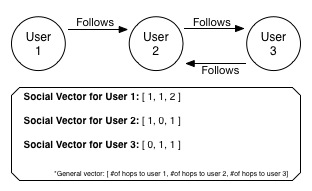
\includegraphics[width=8cm]{images/11_hops_svm.jpg}
  \end{center}
  \caption{Vector describing the number of hops between followers}
  \label{fig:hops}
\end{figure}
% subsubsection social_som (end)
\subsubsection{SOMS Development} % (fold)
\label{ssub:soms_development}
The development and testing of the SOM described in above will be completely independent of the prototype described in Subsection~\ref{sub:web_site_creation}. The SOM training will be made using the datasets described in Subsection~\ref{sub:crawling_twitter} and connection with components from the prototype will be made through the Publish/Subscriber Redis interface. This approach will create an highly modular solution where it will be possible to interact with the trained SOM through terminal where it will be possible to visualize and test results.

% subsubsection soms_development (end)
\subsection{Prototype} % (fold)
\label{sub:web_site_creation}
As described in the report objectives, a prototype will created to demonstrate the project categorizing tweets per topics. The prototype will be developed as a Web Application divided into web server and a client side application that will run on a web browser. The prototype will work in the following way:
\begin{itemize}
  \item A user will be able to login with his twitter id.
  \item The browser will start displaying the user tweets, with the associated topic.
  \item After all the user tweets are displayed, some statistics about the user tweeting topics will be displayed.
\end{itemize}
The wire-frames for the application are provided as attachment, the architecture of the solution can be seen in Figure~\ref{fig:solution} and will be described in the following sub-subsections.
\begin{figure}[tb]
  \begin{center}
    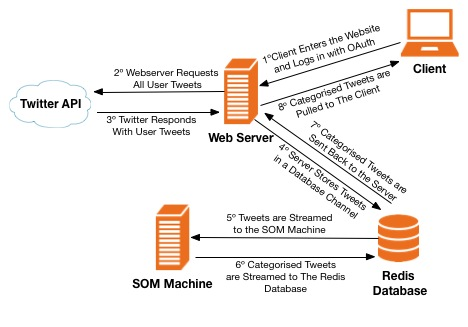
\includegraphics[width=9cm]{images/12_network.jpg}
  \end{center}
  \caption{Topology of the Solution}
  \label{fig:solution}
\end{figure}

\subsubsection{Client Side Application} % (fold)
\label{ssub:client_side_application}
The client side application will be running on the browser of the user connecting to the website. This application is responsible to authenticate itself against the Twitter API, through OAuth, and after that will establish a web-socket channel that will be receiving the categorized tweets as soon as the server dispatches them. The client application will also have to display an interface to the user so he can interact with the application.
% subsubsection client_side_application (end)

\subsubsection{Web Server} % (fold)
\label{ssub:web_server}
The web server will be very simple, since it will only have to get the tweets from the Twitter API and publish them in a channel through the Redis Publish/Subscriber interface, on the other side, the SOM machine will be receiving the Tweets and categorizing them. Also, the web server will have to subscribe to the channel where the SOM Machine is publishing the categorized tweets in order to be able to push them to the client through web-sockets.
% subsubsection web_server (end)

\subsubsection{Redis Database} % (fold)
\label{ssub:redis_database}
The Redis database will be used as a middle man between the Web Server and the SOM Machine as a publish/subscriber system. This is extremely useful because it will separate the login of the web server and web application from the rest of this project. In this way the SOM machine can be running the topic categorization in any programing language while the server can also be working in another language and still be able to contact each other in a simple and efficient way.
% subsubsection redis_database (end)

\subsubsection{SOM Machine} % (fold)
\label{ssub:som_machine}
The SOM Machine is where the Self-Organizing Map trained with the crawled data described in Subsection~\ref{sub:crawling_twitter} will be functioning. It will be subscribing to new tweets sent from the Web Server and will categorize them using the previously trained SOM. After the tweets are categorized they will be published back so the Web Server can deliver them to the client.
% subsubsection som_machine (end)

\subsubsection{Solution Overview} % (fold)
\label{ssub:solution_overview}
We now describe how everything in this solution fits together, based on the diagram in Figure~\ref{fig:solution}. The steps described will be the same, but they will have more detail. For simplicity sake, the OAuth authentication from the client to the twitter API will be omitted since its only objective is to get access to the user tweets.

\begin{itemize}
  \item \textbf{First Step} The client connects to the website through the browser and will login with his twitter account in order for the server be able to download all of his Tweets. When the login process is over it keep an open web-socket with the server in order to receive the categorized tweets.
  \item \textbf{Second and Third Step} The web-server will request all the user tweets through the Twitter API. Twitter will respond with all \footnote{The number of tweets per user are limited to the 3200 most recent through the twitter API} the tweets from the user that logged in.
  \item \textbf{Forth and Fifth Step} The web server will publish the tweets in the Redis database, while subscribing to the channel where the categorized tweets will come out. On the other side the SOM Machine is subscribing to the uncategorized tweets in order to categorize them.
  \item \textbf{Sixth and Seventh Step} After the SOM machine categorizes the tweets it will publish them to the Redis database, which is being subscribed by the web server.
  \item \textbf{Eighth Step} As soon as categorized tweets start hitting the server they will be immediately sent to the client through web sockets. On the client as soon as the categorized tweets hit the browser, they will be injected into the DOM and the user will start to see the tweets that he has made categorized in topics. Lastly after all the tweets have been sent to the browser, some statistics will appear with the amount of tweets per topic throughout the time.
\end{itemize}
% subsubsection solution_overview (end)

% section architecture (end)
 